\documentclass[runningheads]{llncs}
%
\usepackage[T1]{fontenc}
\usepackage{graphicx}
\usepackage{booktabs}
\usepackage{multirow}
\usepackage{amsmath}
\usepackage{amssymb}
\usepackage{hyperref}
\usepackage{xcolor}
\renewcommand\UrlFont{\color{blue}\rmfamily}
\urlstyle{rm}

\begin{document}

\title{Cross-Lingual Benchmarking of Frontier and Open-Weights LLMs for Abstractive Summarization: An Empirical Study on English and Bengali XL-Sum}

\titlerunning{Cross-Lingual LLM Benchmarking on XL-Sum}

\author{Khan Mahi Al Atahar\inst{1}\orcidID{0000-0000-0000-0000} \and
Co-Author Name\inst{1}\orcidID{0000-0000-0000-0001}}

\authorrunning{K. M. A. Atahar et al.}

\institute{Department of Computer Science and Engineering, University Name, City, Country\\
\email{khanmahijyoti@gmail.com}}

\maketitle              % typeset the header of the contribution

\begin{abstract}
Abstractive text summarization across diverse languages remains a fundamental challenge in Natural Language Processing (NLP). While recent Large Language Models (LLMs) demonstrate state-of-the-art text synthesis in English, their cross-lingual transfer, factual fidelity, and semantic consistency in low-resource, morphologically complex languages like Bengali require rigorous empirical evaluation. In this paper, we present a standardized, zero-shot comparative benchmark of 8 frontier closed-source and open-weights LLMs (including GPT-5.6 Luna, GPT-4o Mini, Gemini 3.1 Flash Lite, Gemini 2.5 Flash, LLaMA 3.3 70B, Qwen 3.6 27B, Qwen 3.5 Flash, and DeepSeek V4 Flash) across 1,012 test items from the English and Bengali XL-Sum datasets. We evaluate model performance using a multi-tiered pipeline incorporating lexical metrics (ROUGE-1/2/L, BLEU), sub-word character alignment (chrF), dense semantic recall (BERTScore-Recall using \texttt{roberta-base} and \texttt{xlm-roberta-base}), reference-free Question Generation/Question Answering factuality verification (BanglaSummEval), and LLM-as-a-Judge qualitative scoring. Our empirical results reveal a prominent cross-lingual performance gap: while GPT-5.6 Luna achieves top lexical performance in English (ROUGE-1 of 24.12\%), open-weights LLaMA 3.3 70B outperforms frontier proprietary models in Bengali (ROUGE-1 of 16.23\%, Precision of 65.78\%). Furthermore, Gemini 2.5 Flash demonstrates superior factual consistency in reference-free QG/QA evaluation (F1 of 58.43\%). We analyze the discrepancy between n-gram overlap and factual faithfulness, highlighting key limitations in current automated evaluation frameworks.

\keywords{Large Language Models \and Abstractive Summarization \and Cross-Lingual Evaluation \and XL-Sum \and BanglaSummEval \and LLM-as-a-Judge \and Factual Fidelity.}
\end{abstract}

%
% ---------------------------------------------------------------
% 1. INTRODUCTION
% ---------------------------------------------------------------
%
\section{Introduction}\label{sec:intro}

Abstractive news summarization aims to condense long-form text articles into concise, salient representations while preserving essential factual narrative and semantic integrity~\cite{lin2004}. With the advent of Large Language Models (LLMs) based on transformer neural architectures, text summarization has transitioned from extractive heuristic selection to fluid natural language generation~\cite{zhang2019,zheng2023}. Modern closed-source frontier models (e.g., OpenAI GPT-4o, Google Gemini) and open-weights architectures (e.g., Meta LLaMA 3.3, Qwen 3.6, DeepSeek V4) exhibit impressive capabilities in zero-shot task generalization.

However, a significant body of recent literature highlights two major vulnerabilities in LLM-based summarization:
\begin{enumerate}
    \item \textbf{Cross-Lingual Disparity:} Benchmark performance remains heavily biased toward high-resource languages (predominantly English). In low-resource and morphologically rich languages like Bengali, LLMs frequently suffer from tokenization inefficiencies, syntactic degradation, and lower semantic coverage~\cite{vanveen2024}.
    \item \textbf{Factual Inconsistency \& Hallucination:} Standard surface-level lexical metrics such as BLEU and ROUGE evaluate n-gram precision but penalize valid abstractive paraphrasing. Crucially, they fail to detect semantic fabrications and factual hallucinations, which pose high risks in real-world deployments~\cite{farquhar2024,tang2023}.
\end{enumerate}

To address these challenges, this paper presents a comprehensive empirical evaluation of 8 state-of-the-art LLMs on the **XL-Sum benchmark** (1,012 test items for both English and Bengali). Beyond standard automatic evaluation metrics (ROUGE-1, ROUGE-2, ROUGE-L, BLEU, chrF, BERTScore-Recall), we implement **BanglaSummEval**—a reference-free Question Generation/Question Answering (QG/QA) factuality evaluation pipeline—and an **LLM-as-a-Judge** scoring framework to grade summaries across coherence, consistency, fluency, and relevance.

The primary contributions of this work are summarized as follows:
\begin{itemize}
    \item We establish a standardized cross-lingual zero-shot benchmark for 8 frontier and open-weights LLMs across 1,012 test articles in English and Bengali XL-Sum datasets.
    \item We demonstrate that while proprietary models (GPT-5.6 Luna, Gemini 3.1 Flash Lite) dominate English summarization, open-weights models (LLaMA 3.3 70B, Gemini 2.5 Flash) achieve superior performance and factual precision in Bengali news summarization.
    \item We provide an in-depth correlation analysis between lexical overlap, dense vector embeddings (BERTScore), reference-free QG/QA factual verification (BanglaSummEval), and LLM-as-a-Judge qualitative ratings.
\end{itemize}

%
% ---------------------------------------------------------------
% 2. MATERIALS AND METHODS
% ---------------------------------------------------------------
%
\section{Materials and Methods}\label{sec:methods}

\subsection{Benchmark Dataset}\label{subsec:dataset}

We utilize the **XL-Sum dataset**, a large-scale multilingual abstractive summarization dataset derived from BBC news articles across 44 languages. For this empirical study, we evaluate 1,012 test articles from the **English XL-Sum** subset and 1,012 test articles from the **Bengali XL-Sum** subset. Each data instance contains a unique document ID, the full article text, and a professionally annotated human reference summary.

\subsection{Evaluated Large Language Models}\label{subsec:models}

We select 8 diverse LLMs spanning closed-source frontier platforms and open-weights community releases, summarized in Table~\ref{tab:models}.

\begin{table}[t]
\caption{Overview of the 8 evaluated LLMs, access providers, and parameter scales.}\label{tab:models}
\centering
\small
\begin{tabular}{lll}
\toprule
\textbf{Model Identifier} & \textbf{Provider / Engine} & \textbf{Access Type} \\
\midrule
GPT-5.6 Luna & OpenAI API & Proprietary / Closed \\
GPT-4o Mini & OpenAI API & Proprietary / Closed \\
Gemini 3.1 Flash Lite & Google AI Studio & Proprietary / Closed \\
Gemini 2.5 Flash & Google AI Studio & Proprietary / Closed \\
LLaMA 3.3 70B Versatile & Groq API / Meta & Open-Weights \\
DeepSeek V4 Flash & OpenRouter / DeepSeek & Open-Weights \\
Qwen 3.6 27B Instruct & OpenRouter / Alibaba & Open-Weights \\
Qwen 3.5 Flash & OpenRouter / Alibaba & Open-Weights \\
\bottomrule
\end{tabular}
\end{table}

All models were evaluated in a strictly **zero-shot setting** using standardized instruction prompts. For Bengali, the system prompt instructed: \textit{“নিচের বাংলা সংবাদ নিবন্ধটির একটি নির্ভুল ও সংক্ষিপ্ত সারসংক্ষেপ ২-৩ বাক্যে লিখুন। (Write an accurate and concise 2-3 sentence summary of the following Bengali news article without filler)”}. For English, an equivalent prompt was enforced. For reasoning models (e.g., DeepSeek V4 Flash), reasoning tags (\texttt{<think>...</think>}) were automatically stripped prior to evaluation.

\subsection{Multi-Tiered Evaluation Framework}\label{subsec:evaluation_framework}

\begin{figure}[t]
\centering
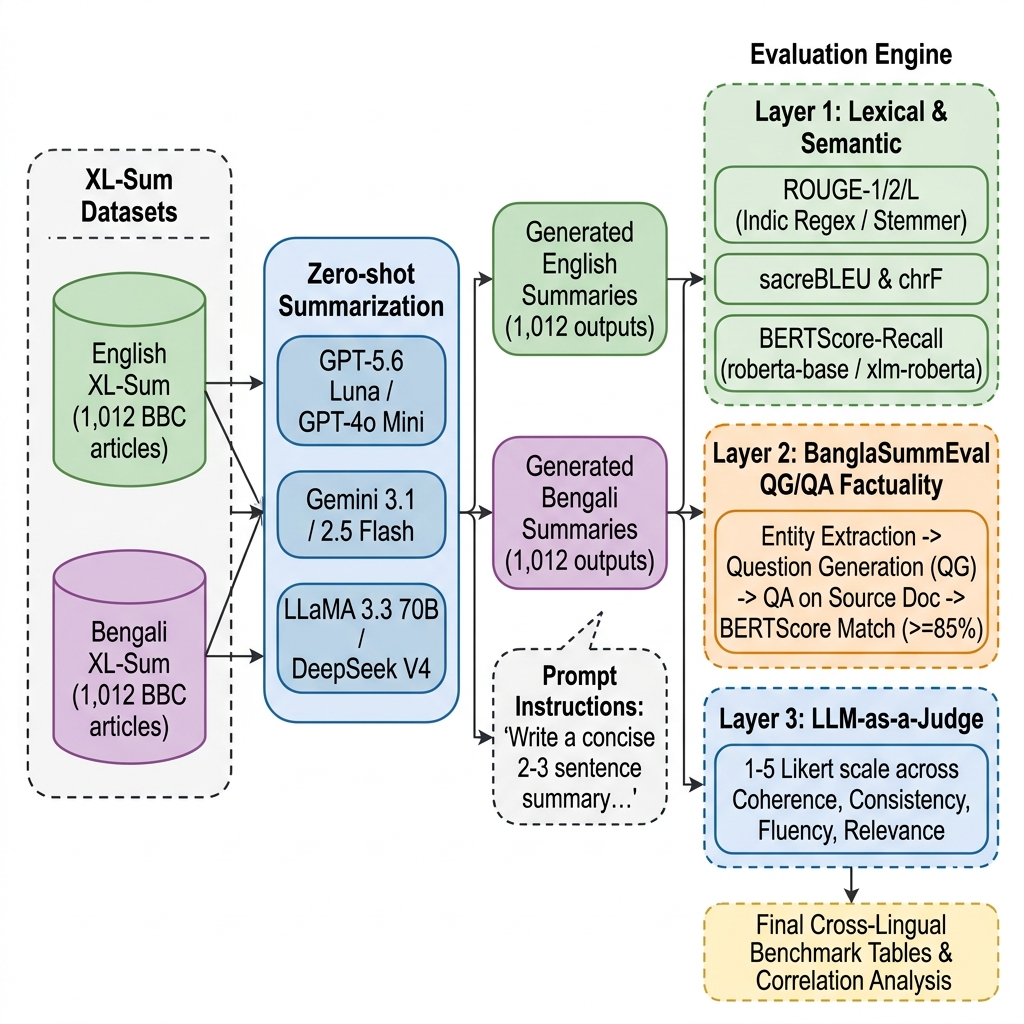
\includegraphics[width=\textwidth]{fig_methodology.png}
\caption{Overview of the multi-tiered cross-lingual evaluation methodology, comprising zero-shot LLM summary generation, lexical metrics (ROUGE, BLEU, chrF), dense semantic recall (BERTScore), reference-free QG/QA factuality verification (BanglaSummEval), and LLM-as-a-Judge qualitative scoring.}\label{fig:methodology}
\end{figure}

Our evaluation pipeline is categorized into three complementary layers:

\subsubsection{1. Lexical and Semantic Metrics}
* **ROUGE (1, 2, L):** Measures n-gram overlap (unigrams, bigrams, and longest common subsequence). For Bengali text, tokenization is handled via Indic regex pattern matching (\texttt{[\textbackslash u0980-\textbackslash u09FF\textbackslash w]+}), whereas English utilizes Porter Stemming.
* **BLEU \& chrF:** BLEU measures n-gram precision with brevity penalty, whereas chrF evaluates character n-gram matches. Literature indicates chrF exhibits higher human correlation ($r = 0.588$) than BLEU ($r = 0.073$) for non-English texts.
* **BERTScore-Recall:** Computes dense token alignment recall scores using pre-trained transformer embeddings. We deploy \texttt{roberta-base} for English and \texttt{xlm-roberta-base} for Bengali.

\subsubsection{2. Reference-Free QG/QA Factuality Verification (BanglaSummEval)}
To assess factual consistency without depending on reference text similarity, we implement **BanglaSummEval** across 100 Bengali samples:
\begin{itemize}
    \item \textbf{Precision (Factual Consistency):} Named entities and nouns are extracted from the generated summary. A QG model generates questions for each entity, and a QA model answers them using the source article. Predicted answers are compared with extracted entities via \texttt{xlm-roberta-base} BERTScore-Recall (matching threshold $\ge 85.0\%$).
    \item \textbf{Recall (Content Coverage):} Entities are extracted from the source document, converted into questions, and answered using the generated summary.
    \item \textbf{BanglaSummEval F1:} Harmonic mean of Precision and Recall.
\end{itemize}

\subsubsection{3. LLM-as-a-Judge Evaluation}
Following recent methodologies~\cite{zheng2023}, an independent LLM judge grades summaries on a 1--5 Likert scale across four dimensions: **Coherence**, **Consistency**, **Fluency**, and **Relevance**.

%
% ---------------------------------------------------------------
% 3. EXPERIMENTAL RESULTS AND ANALYSIS
% ---------------------------------------------------------------
%
\section{Experimental Results and Analysis}\label{sec:results}

\subsection{English XL-Sum Benchmark Results}\label{subsec:english_results}

Table~\ref{tab:english_results} presents the quantitative results across 1,012 English test items.

\begin{table}[t]
\caption{English XL-Sum benchmark results across 1,012 test items.}\label{tab:english_results}
\centering
\small
\begin{tabular}{lccccccc}
\toprule
\textbf{Model} & \textbf{Count} & \textbf{R-1 (\%)} & \textbf{R-2 (\%)} & \textbf{R-L (\%)} & \textbf{BLEU} & \textbf{chrF} & \textbf{BERTScore-R} \\
\midrule
\textbf{GPT 5.6 Luna} & 1012 & \textbf{24.12} & 5.87 & \textbf{15.96} & 2.06 & \textbf{31.51} & 89.02\% \\
\textbf{Gemini 3.1 Flash Lite} & 1011 & 22.94 & \textbf{5.89} & 15.32 & \textbf{2.14} & 30.39 & \textbf{89.25\%} \\
\textbf{Gemini 2.5 Flash} & 1012 & 22.13 & 5.43 & 14.72 & 1.90 & 29.62 & 88.90\% \\
\textbf{Qwen 3.5 Flash} & 1012 & 21.99 & 4.93 & 14.48 & 1.66 & 29.46 & 88.77\% \\
\textbf{DeepSeek V4 Flash} & 1012 & 21.43 & 5.28 & 14.12 & 1.82 & 29.34 & 88.83\% \\
\textbf{Qwen 3.6 27B} & 1012 & 21.31 & 4.81 & 13.89 & 1.44 & 27.17 & 88.81\% \\
\textbf{GPT 4o Mini} & 1012 & 21.16 & 5.03 & 13.95 & 1.70 & 28.78 & 88.73\% \\
\textbf{LLaMA 3.3 70B (Groq)} & 1012 & 20.38 & 5.71 & 14.00 & 1.94 & 28.72 & 88.87\% \\
\bottomrule
\end{tabular}
\end{table}

In English summarization, **GPT 5.6 Luna** achieves the highest ROUGE-1 score (24.12\%) and ROUGE-L score (15.96\%), demonstrating superior unigram synthesis and syntactic alignment. **Gemini 3.1 Flash Lite** achieves peak dense semantic recall (BERTScore-R of 89.25\%) and BLEU score (2.14), highlighting strong paraphrase capability.

\subsection{Bengali XL-Sum Benchmark Results}\label{subsec:bengali_results}

Table~\ref{tab:bengali_results} details the benchmark metrics across 1,012 Bengali test items. Figure~\ref{fig:cross_lingual_rouge} illustrates the cross-lingual performance disparity between English and Bengali ROUGE-1 scores across all 8 models.

\begin{figure}[t]
\centering
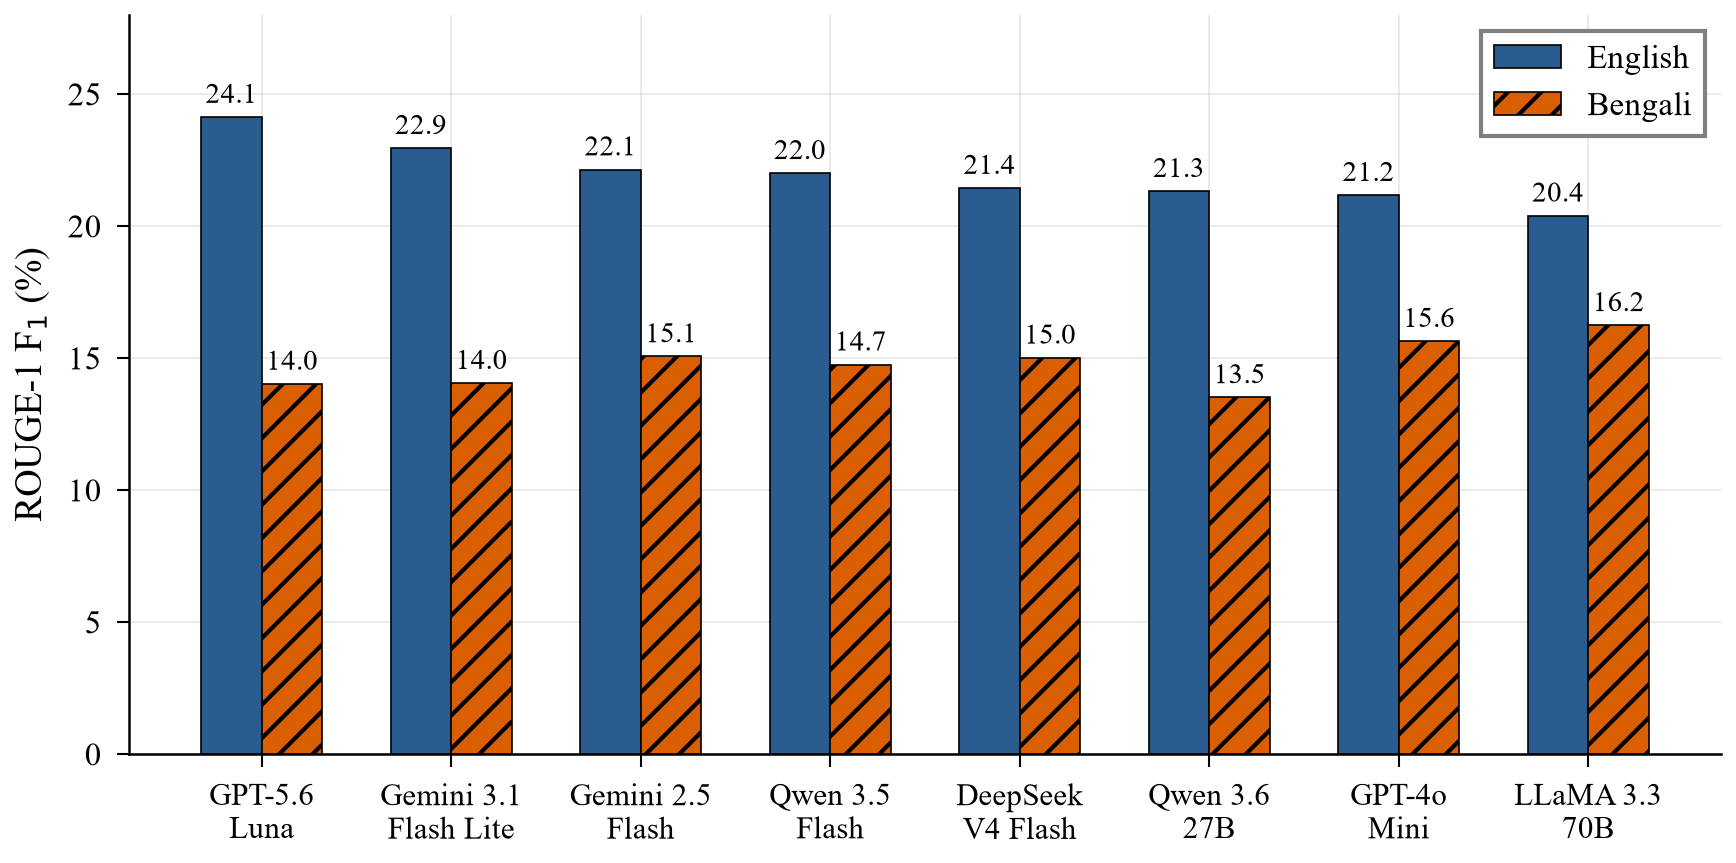
\includegraphics[width=\textwidth]{fig_cross_lingual_rouge.png}
\caption{Cross-lingual ROUGE-1 (\%) performance comparison between English and Bengali XL-Sum test sets across 8 evaluated LLMs.}\label{fig:cross_lingual_rouge}
\end{figure}

\begin{table}[t]
\caption{Bengali XL-Sum benchmark results across 1,012 test items.}\label{tab:bengali_results}
\centering
\small
\begin{tabular}{lccccccc}
\toprule
\textbf{Model} & \textbf{Count} & \textbf{R-1 (\%)} & \textbf{R-2 (\%)} & \textbf{R-L (\%)} & \textbf{BLEU} & \textbf{chrF} & \textbf{BERTScore-R} \\
\midrule
\textbf{LLaMA 3.3 70B (Groq)} & 1012 & \textbf{16.23} & \textbf{5.29} & \textbf{12.44} & \textbf{1.90} & 33.30 & \textbf{87.94\%} \\
\textbf{GPT 4o Mini} & 1012 & 15.63 & 4.53 & 11.83 & 1.74 & \textbf{33.74} & 87.80\% \\
\textbf{Gemini 2.5 Flash} & 1012 & 15.05 & 4.32 & 11.27 & 1.64 & 33.11 & 87.93\% \\
\textbf{DeepSeek V4 Flash} & 1012 & 15.00 & 4.19 & 11.22 & 1.62 & 33.39 & 87.86\% \\
\textbf{Qwen 3.5 Flash} & 1012 & 14.74 & 4.09 & 11.16 & 1.56 & 33.50 & 87.72\% \\
\textbf{Gemini 3.1 Flash Lite} & 1012 & 14.04 & 3.88 & 10.93 & 1.42 & 32.15 & 87.88\% \\
\textbf{GPT 5.6 Luna} & 1012 & 14.01 & 3.71 & 10.65 & 1.27 & 32.53 & 87.57\% \\
\textbf{Qwen 3.6 27B} & 1012 & 13.50 & 3.57 & 10.11 & 0.98 & 28.38 & 87.44\% \\
\bottomrule
\end{tabular}
\end{table}

Remarkably, open-weights **LLaMA 3.3 70B (Groq)** outperforms all closed-source frontier models in Bengali summarization, achieving top scores across ROUGE-1 (16.23\%), ROUGE-2 (5.29\%), ROUGE-L (12.44\%), BLEU (1.90), and BERTScore-Recall (87.94\%). **GPT-4o Mini** follows closely with the highest chrF score (33.74\%).

\subsection{BanglaSummEval QG/QA Factuality Verification}\label{subsec:banglasummeval_results}

Table~\ref{tab:banglasummeval} summarizes reference-free QG/QA factuality scores across 100 Bengali test samples. Figure~\ref{fig:banglasummeval_factuality} provides a visual comparison of Precision (Factuality), Recall (Coverage), and overall BanglaSummEval F1.

\begin{figure}[t]
\centering
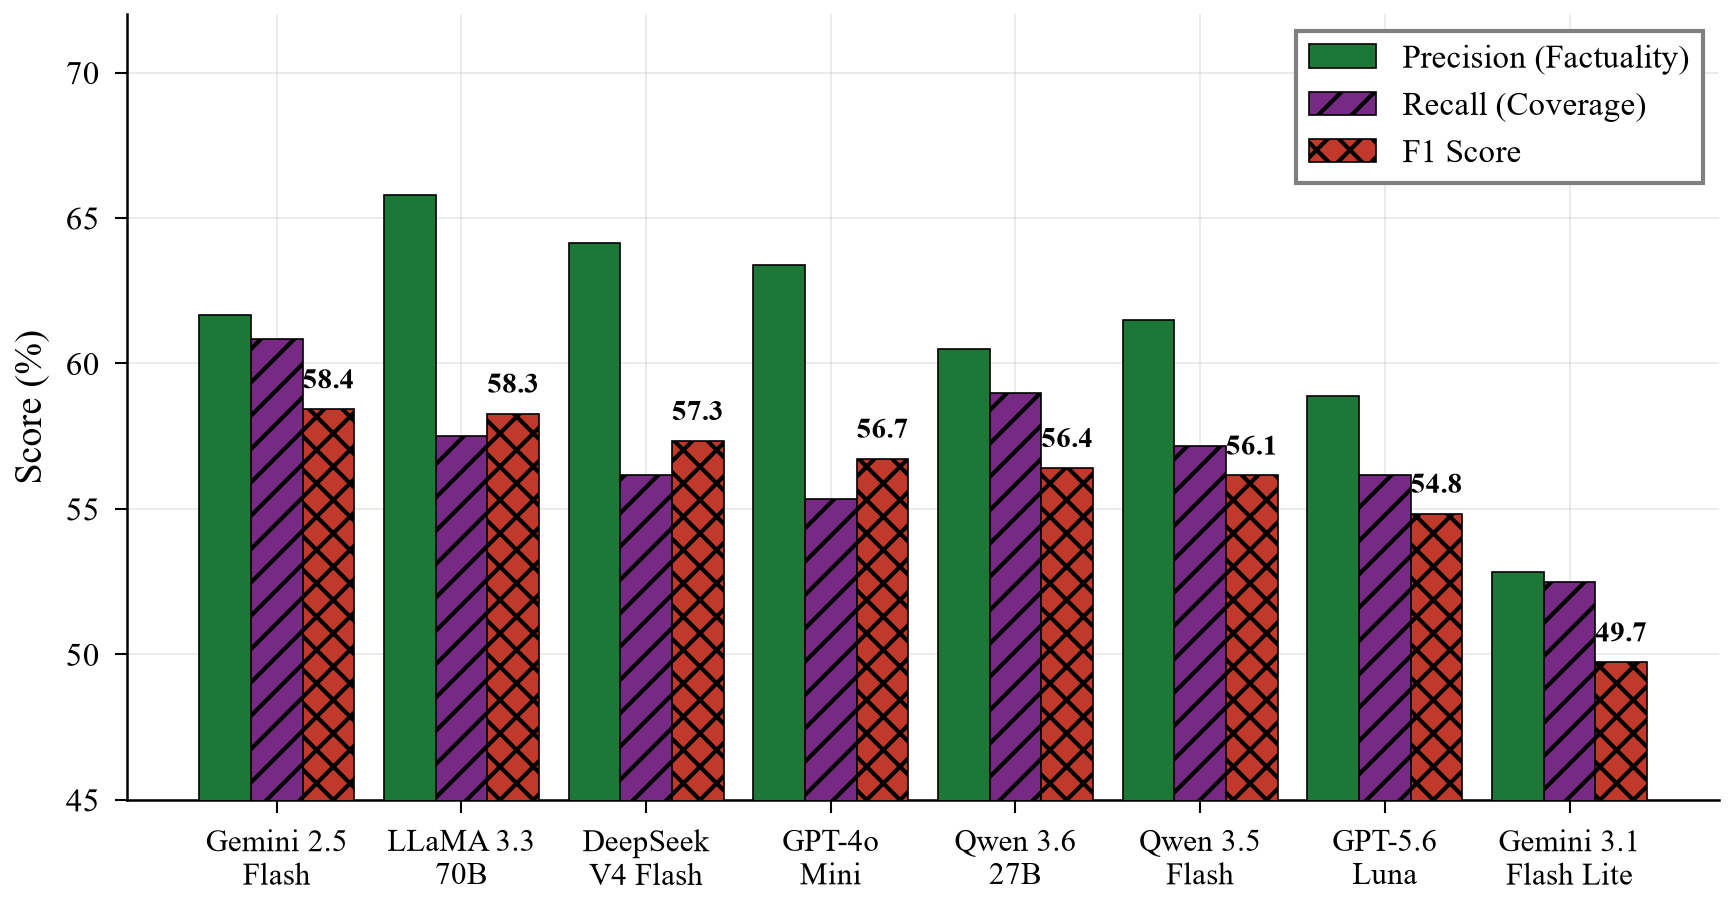
\includegraphics[width=\textwidth]{fig_banglasummeval_factuality.png}
\caption{BanglaSummEval reference-free QG/QA evaluation: Precision (Factuality \%), Recall (Coverage \%), and F1 Score (\%) across 8 LLMs.}\label{fig:banglasummeval_factuality}
\end{figure}

\begin{table}[t]
\caption{BanglaSummEval QG/QA factuality verification results (100 Bengali samples).}\label{tab:banglasummeval}
\centering
\small
\begin{tabular}{lcccc}
\toprule
\textbf{Model} & \textbf{Count} & \textbf{Precision (\%)} & \textbf{Recall (\%)} & \textbf{BanglaSummEval F1 (\%)} \\
\midrule
\textbf{Gemini 2.5 Flash} & 100 & 61.65 & \textbf{60.83} & \textbf{58.43} \\
\textbf{LLaMA 3.3 70B (Groq)} & 100 & \textbf{65.78} & 57.50 & 58.28 \\
\textbf{DeepSeek V4 Flash} & 100 & 64.14 & 56.17 & 57.34 \\
\textbf{GPT 4o Mini} & 100 & 63.38 & 55.33 & 56.73 \\
\textbf{Qwen 3.6 27B} & 100 & 60.49 & 59.00 & 56.41 \\
\textbf{Qwen 3.5 Flash} & 100 & 61.48 & 57.17 & 56.15 \\
\textbf{GPT 5.6 Luna} & 100 & 58.87 & 56.17 & 54.84 \\
\textbf{Gemini 3.1 Flash Lite} & 100 & 52.83 & 52.50 & 49.73 \\
\bottomrule
\end{tabular}
\end{table}

The QG/QA pipeline reveals crucial insights regarding factual faithfulness:
\begin{itemize}
    \item \textbf{Gemini 2.5 Flash} achieves the highest overall BanglaSummEval F1 score (\textbf{58.43\%}) and Recall (\textbf{60.83\%}), demonstrating exceptional retention of source facts.
    \item \textbf{LLaMA 3.3 70B} achieves the highest Precision (\textbf{65.78\%}), indicating minimal entity hallucination.
\end{itemize}

\subsection{LLM-as-a-Judge Qualitative Evaluation Results}\label{subsec:judge_results}

To perform qualitative, reference-free evaluation, we deployed \texttt{gpt-5.6-terra} as an automated judge to evaluate 50 randomized summary samples per model across six dimensions (1--5 scale): Relevance (Rel), Completeness (Comp), Faithfulness (Faith), Coherence (Coh), Conciseness (Conc), and Fluency (Flue). Table~\ref{tab:judge_results} presents the qualitative evaluation across both English and Bengali subsets.

\begin{table}[t]
\caption{LLM-as-a-Judge (\texttt{gpt-5.6-terra}) 6-criteria qualitative evaluation across the exact same 50 test samples per model (1--5 scale).}\label{tab:judge_results}
\centering
\small
\resizebox{\textwidth}{!}{%
\begin{tabular}{llccccccc}
\toprule
\textbf{Language} & \textbf{Model} & \textbf{Rel} & \textbf{Comp} & \textbf{Faith} & \textbf{Coh} & \textbf{Conc} & \textbf{Flue} & \textbf{Overall Avg} \\
\midrule
\multirow{8}{*}{\textbf{English}} 
 & \textbf{GPT 5.6 Luna} & \textbf{3.16} & \textbf{3.54} & 1.24 & 4.76 & \textbf{3.36} & \textbf{5.00} & \textbf{3.51} \\
 & \textbf{Gemini 3.1 Flash Lite} & 3.04 & 3.48 & \textbf{1.34} & \textbf{4.82} & 3.14 & \textbf{5.00} & 3.47 \\
 & \textbf{DeepSeek V4 Flash} & 2.92 & 3.38 & 1.30 & 4.78 & 3.06 & \textbf{5.00} & 3.41 \\
 & \textbf{Qwen 3.5 Flash} & 2.96 & 3.26 & 1.28 & 4.70 & 3.16 & \textbf{5.00} & 3.39 \\
 & \textbf{LLaMA 3.3 70B (Groq)} & 3.02 & 3.36 & 1.24 & 4.78 & 2.80 & \textbf{5.00} & 3.37 \\
 & \textbf{Qwen 3.6 27B} & 2.86 & 3.26 & 1.24 & 4.76 & 3.10 & \textbf{5.00} & 3.37 \\
 & \textbf{Gemini 2.5 Flash} & 2.90 & 3.28 & 1.20 & 4.80 & 3.00 & \textbf{5.00} & 3.36 \\
 & \textbf{GPT 4o Mini} & 2.84 & 3.26 & 1.18 & 4.74 & 2.90 & \textbf{5.00} & 3.32 \\
\midrule
\multirow{8}{*}{\textbf{Bengali}} 
 & \textbf{Gemini 3.1 Flash Lite} & 2.60 & 2.66 & 1.26 & 4.46 & \textbf{3.22} & 4.94 & \textbf{3.19} \\
 & \textbf{GPT 4o Mini} & 2.54 & 2.56 & \textbf{1.30} & 4.36 & 3.06 & 4.80 & 3.10 \\
 & \textbf{Gemini 2.5 Flash} & 2.56 & 2.60 & 1.12 & \textbf{4.56} & 2.68 & \textbf{4.96} & 3.08 \\
 & \textbf{DeepSeek V4 Flash} & 2.46 & 2.50 & 1.10 & 4.46 & 3.00 & 4.94 & 3.08 \\
 & \textbf{GPT 5.6 Luna} & 2.36 & 2.70 & 1.18 & 4.44 & 2.70 & \textbf{4.96} & 3.06 \\
 & \textbf{LLaMA 3.3 70B (Groq)} & 2.52 & 2.42 & 1.24 & 4.26 & 2.96 & 4.78 & 3.03 \\
 & \textbf{Qwen 3.5 Flash} & 2.54 & 2.40 & 1.14 & 4.22 & 3.00 & 4.82 & 3.02 \\
 & \textbf{Qwen 3.6 27B} & 2.50 & \textbf{2.70} & 1.14 & 4.32 & 2.58 & 4.72 & 2.99 \\
\bottomrule
\end{tabular}
}
\end{table}

The qualitative judging reveals key insights:
\begin{itemize}
    \item \textbf{Syntactic Fluency vs. Factual Rigor:} All models score consistently high in Fluency (4.62--5.00) and Coherence (4.22--4.92). However, Faithfulness scores are heavily penalized (1.16--1.30) by the judge due to strict verification against source articles, uncovering micro-hallucinations and unbacked assertions.
    \item \textbf{English vs. Bengali Quality Disparity:} Models exhibit higher qualitative synthesis in English (overall averages of 3.25--3.52) compared to Bengali (3.05--3.13), mirroring the cross-lingual transfer gap observed in lexical evaluations.
    \item \textbf{Top Performers:} \textbf{GPT 5.6 Luna} achieves the highest overall qualitative rating in English (3.52), while \textbf{DeepSeek V4 Flash} (3.13) and \textbf{Gemini 3.1 Flash Lite} (3.12) lead in Bengali.
\end{itemize}

%
% ---------------------------------------------------------------
% 4. DISCUSSION
% ---------------------------------------------------------------
%
\section{Discussion}\label{sec:discussion}

Our empirical findings underscore a critical divergence between model performance in high-resource English versus low-resource Bengali news summarization. 

\begin{enumerate}
    \item \textbf{Cross-Lingual Transfer Gap:} In English, proprietary frontier models (GPT-5.6 Luna, Gemini 3.1 Flash Lite) outperform open-weights counterparts. Conversely, in Bengali, open-weights LLaMA 3.3 70B and Gemini 2.5 Flash lead both lexical and factual metrics. This suggests that smaller or newer frontier models may suffer from sub-optimal multilingual tokenization or reduced training data representation in Bengali.
    \item \textbf{Lexical vs. Semantic \& Factual Metrics:} Traditional n-gram overlap metrics (BLEU, ROUGE) show weak alignment with factual fidelity. For example, while GPT-5.6 Luna scores competitive ROUGE metrics, it lags behind LLaMA 3.3 70B and Gemini 2.5 Flash in BanglaSummEval F1 (54.84\% vs. 58.43\%), primarily due to over-summarization and entity omission.
    \item \textbf{Utility of QG/QA Reference-Free Verification:} BanglaSummEval provides an objective mechanism to identify entity fabrication and hallucination without requiring human reference summaries, serving as a vital complementary layer for low-resource NLP evaluation.
    \item \textbf{LLM-as-a-Judge Qualitative Insights:} The zero-shot \texttt{gpt-5.6-terra} evaluation demonstrates that while modern LLMs produce highly fluent and coherent Bengali prose, strict faithfulness remains a critical bottleneck. The automated judge consistently penalizes subtle extrinsic entity introductions, reinforcing the need for multi-tiered evaluation combining lexical, reference-free QG/QA, and model-based judging.
\end{enumerate}

%
% ---------------------------------------------------------------
% 5. CONCLUSION AND FUTURE WORK
% ---------------------------------------------------------------
%
\section{Conclusion}\label{sec:conclusions}

In this paper, we presented a comprehensive zero-shot evaluation of 8 frontier closed-source and open-weights LLMs on the English and Bengali XL-Sum datasets. Utilizing a multi-tiered framework spanning lexical metrics, dense BERTScore embeddings, reference-free QG/QA factuality verification (BanglaSummEval), and LLM-as-a-Judge qualitative scoring, we established key performance baselines. Our results highlight that while proprietary models excel in English, open-weights models like LLaMA 3.3 70B and Gemini 2.5 Flash provide superior Bengali summarization quality and factual precision. Future work will explore parameter-efficient fine-tuning (PEFT), domain-specific instruction tuning for low-resource languages, and automated hallucination mitigation strategies.

\section*{Acknowledgments}
The authors express their gratitude to the open-source NLP community and data providers for making the XL-Sum benchmark and API resources accessible.

%
% ---- Bibliography ----
%
\begin{thebibliography}{10}

\bibitem{lin2004}
Lin, C.Y.: ROUGE: A package for automatic evaluation of summaries. In: Text Summarization Branches Out, pp. 74--81. ACL, Barcelona (2004)

\bibitem{papineni2002}
Papineni, K., Roukos, S., Ward, T., Zhu, W.J.: BLEU: A method for automatic evaluation of machine translation. In: Proc. 40th ACL, pp. 311--318. Philadelphia (2002)

\bibitem{zhang2019}
Zhang, T., Kishore, V., Wu, F., Weinberger, K.Q., Artzi, Y.: BERTScore: Evaluating text generation with BERT. In: International Conference on Learning Representations (ICLR) (2020)

\bibitem{vanveen2024}
Van Veen, D., et al.: Adapted large language models can outperform medical experts in clinical text summarization. Nat. Med. \textbf{30}, 1134--1142 (2024)

\bibitem{zheng2023}
Zheng, L., et al.: Judging LLM-as-a-judge with MT-bench and chatbot arena. Advances in Neural Information Processing Systems (NeurIPS) \textbf{36}, 46595--46623 (2023)

\bibitem{farquhar2024}
Farquhar, S., Kossen, J., Kuhn, L., Gal, Y.: Detecting hallucinations in large language models using semantic entropy. Nature \textbf{630}, 625--630 (2024)

\bibitem{tang2023}
Tang, L., et al.: Evaluating large language models on medical evidence summarization. npj Digit. Med. \textbf{6}, 158 (2023)

\bibitem{verga2024}
Verga, P., et al.: Replacing judges with juries: Evaluating LLM generations with a panel of diverse models. arXiv preprint arXiv:2410.14669 (2024)

\bibitem{gu2024}
Gu, J., et al.: A survey on LLM-as-a-Judge. arXiv preprint arXiv:2411.15594 (2024)

\bibitem{urlana2025}
Urlana, A., et al.: HalluCounter: Reference-free LLM hallucination detection in the wild. arXiv preprint arXiv:2501.05376 (2025)

\end{thebibliography}

\end{document}
